\documentclass{article}
\usepackage[utf8]{inputenc}
\usepackage[UKenglish]{babel}
\usepackage[UKenglish]{isodate}
\usepackage{fullpage}
\usepackage{amsthm}
\usepackage{amsfonts}
\usepackage{amsmath}
\usepackage{mathtools}
\usepackage{hyperref}
\usepackage[capitalise]{cleveref}
\usepackage{bm}
\usepackage{booktabs}
\usepackage{tikz}
\usepackage{xcolor}
\usepackage[backgroundcolor=lightgray]{todonotes}
\usepackage{complexity}
\usepackage{soul}
\usepackage[ruled,vlined]{algorithm2e}
\usepackage{subcaption}

\newtheorem{theorem}{Theorem}
\newtheorem{lemma}[theorem]{Lemma}
\newtheorem{proposition}[theorem]{Proposition}
\newtheorem{corollary}[theorem]{Corollary}
\newtheorem{conjecture}[theorem]{Conjecture}
\theoremstyle{definition}
\newtheorem{definition}[theorem]{Definition}
\newtheorem{example}[theorem]{Example}
\theoremstyle{remark}
\newtheorem*{remark}{Remark}

\Crefname{property}{Property}{Properties}
\Crefname{condition}{Condition}{Conditions}
\creflabelformat{condition}{#2(#1)#3}

\DeclareMathOperator{\WMC}{WMC}
\DeclareMathOperator{\nWMC}{NWMC}
\DeclareMathOperator{\id}{id}
\DeclareMathOperator{\End}{End}
\DeclareMathOperator{\im}{im}

\usetikzlibrary{cd}
\usetikzlibrary{bayesnet}
\usetikzlibrary{calc}

\tikzset{
  Subset/.style={
    draw=none,
    every to/.append style={
      edge node={node [sloped, allow upside down, auto=false]{$\subset$}}}
  }
}

\title{Weighted Model Counting with Conditional Probabilities}
\author{Paulius Dilkas}

\begin{document}
\maketitle

\section{Introduction}

\paragraph{Legend.}
\begin{description}
\item[F] Feedback (round 1).
\item[F2] Feedback (round 2).
\item[FP] Feedback from the review panel.
\item[\textbullet] My own idea.
\end{description}

\paragraph{The big TODO list.}
\begin{itemize}
\item Look into ways to theoretically justify the performance benefits. Some
  suggestions:
  \begin{itemize}
  \item the number of variables,
  \item the number of clauses/CPTs/lines in CPTs,
  \item the proportion of edges that exist,
  \item average degree,
  \item average number of clauses that a variable is in,
  \item the number of clusters in the linear/tree-like decomposition.
  \end{itemize}
\item Have an example of how the ADDs function in this situation. If not for the
  paper, then at least for slides. Use the framework to check its correctness.
\item[F] Give a concrete example of something impossible to represent using WMC.
\item Turn the saved PDFs into citations.
\item[F] What are the main claims, what are the main takeaways, intuitive [???]
  of theorems to follow. To do this, we appeal to algebraic constructions to
  define the main concepts for introducing measures on Boolean algebras.
\item[F] Can you say something here about factorized vs non-factorized
  weight function definitions? That is, factorized is when $w$ maps literals to
  $R_{\ge 0}$, non-factorized is when $w$ maps models to $R_{\ge 0}$ and
  \begin{itemize}
  \item come up with nice example when non-factorized weights are intuitive;
  \item clarify that the factorized definition have is w.r.t. models, in case some
    one gets confused. [It doesn't have to be, if the BA is not free---P.]
  \end{itemize}
\item[F2] The paper at this stage is very technical---the danger is that WMC/SRL
  people may not be able to follow it and so would be hard to get accepted.
  Without clear target audience, [???] get work accepted. My main high level
  suggestion is that let us tease apart what you have and see if a story
  emerges. That is, let us attempt to write a paper {\bf with examples} and
  see whether with significant motivation, we have a story emerging. Below,
  sample text needed to adequately motivate [???] for WMC/SRL community.
\item[FP] Clear up questions about independence between literals.
\item[F2] Preliminaries: explain with examples: models $=$ elements [atoms] of
  algebra.
\item WMC as a Measure
  \begin{itemize}
  \item[F2] Need to explain how WMC and NWMC connects to standard definitions of
    WMC and $\Pr(\phi \mid e) = \WMC(\phi \land e)/\WMC(e)$.
  \item[F2] You need to explain what precisely these mean in logic and models
    and weight functions are usually defined and understood.
  \item Be careful about mentioning ideals, filters, and quotients.
  \end{itemize}
\item What Measures are WMC-Definable: proofs need to be updated and
  propositions could be phrased in a better way, but the gist should be the
  same.
\item Extending the Algebra.
  \begin{itemize}
  \item[F2] If you prove (b) above, you could motivate why weights on literals
    is attractive and whether there is a way to augment the expressivity of WMC
    while still maintaining literal level weights. Hence this action.
  \item[F2] You need to explain the significance of this result.
  \end{itemize}
\item Make up my mind about $a, b$ vs. $x, y$ and stick to it (maybe $x, y$?).
\item Terminology: `with generating set $S$' $\to$ `over $S$'.
\item Perhaps reorder the section of preliminaries into paragraphs, i.e., a
  paragraph for order, for homomorphisms, etc. This would take up less space.
\item Notation: if $L$ denotes literals, then it doesn't denote a generating
  set.
\item Prove that we have an algebra of functions with two (?) additional
  operations. Or maybe just cite the original paper for this.
\item The function $\phi$ created by the algorithm can be seen as a measure on
  the BA $2^U$. Can I at least show that this BA has fewer elements as a measure
  of compactness w.r.t. the measure?
\item Note that we're going to use logical notation for BAs. Give an example of
  the two notations.
\item Could clarify why $[\lambda_{X=0}] = \overline{[\lambda_{X=1}]}$. This
  follows from the definition. Or should I avoid the overline notation?
\item After the experiments are finished, note the processor, memory per thread,
  and add the following acknowledgment. This work has made use of the resources
  provided by the Edinburgh Compute and Data Facility (ECDF)
  (\url{http://www.ecdf.ed.ac.uk/}).
\end{itemize}

\paragraph{Experimental setup.}
\begin{itemize}
\item
  Algorithms\footnote{\url{http://beyondnp.org/pages/solvers/model-counters-exact/}}
  \begin{itemize}
  \item ADDMC \cite{DBLP:conf/aaai/DudekPV20} (rediscovered the
    multiplicativity of BAs in different words) (with optimal settings)
  \item Cachet \cite{DBLP:conf/sat/SangBBKP04}
  \item c2d \cite{DBLP:conf/ecai/Darwiche04}
  \item d4 \cite{DBLP:conf/ijcai/LagniezM17} (closed source, boo!)
  \item miniC2D  \cite{DBLP:conf/ijcai/OztokD15}
  \end{itemize}
\item Encodings:
  \begin{itemize}
  \item \texttt{-d02} \cite{DBLP:conf/kr/Darwiche02}
  \item \texttt{-sbk05} \cite{DBLP:conf/aaai/SangBK05}
  \item \texttt{-cd05} \cite{DBLP:conf/ijcai/ChaviraD05}
  \item \texttt{-cd06} \cite{DBLP:conf/sat/ChaviraD06} (supposed to be the best)
  \item mine
  \end{itemize}
  All except mine are from Ace
  3.0\footnote{\url{http://reasoning.cs.ucla.edu/ace/}} and should be compiled
  with \texttt{-encodeOnly} (i.e., don't compile the CNF into an AC) and
  \texttt{-noEclause} (i.e., only use standard syntax) flags.
\item Datasets\footnote{There might be more at
    \url{https://meelgroup.github.io/}.}
  \begin{itemize}
  \item binary Bayesian networks from Sang et
    al.\footnote{\url{https://www.cs.rochester.edu/u/kautz/Cachet/}}
    \cite{DBLP:conf/aaai/SangBK05}
    \begin{itemize}
    \item Grid (networks) (ratio 75 means that 75\% of the nodes are
      deterministic),
    \item Plan recognition (problems),
    \item Deterministic quick medical reference (what do the numbers mean? the
      README doesn't say).
    \end{itemize}
  \item Bayesian networks available with Ace
    \begin{itemize}
    \item \texttt{2004-pgm} \cite{DBLP:journals/ijar/ChaviraDJ06} (binary)
    \item \texttt{2005-ijcai} \cite{DBLP:conf/ijcai/ChaviraD05}. The Genie/Smile
      files have their own citation data that I should probably extract. This is
      the only dataset that has some non-binary networks.
    \item \texttt{2006-ijar} \cite{DBLP:journals/ijar/ChaviraDJ06} (binary)
    \end{itemize}
  \item ProbLog \cite{DBLP:conf/uai/FierensBTGR11}
  \item probabilistic programs \cite{DBLP:journals/corr/abs-2005-09089}
  \end{itemize}
\end{itemize}

\paragraph{Contributions.}
\begin{itemize}
\item WMC defines a measure over a BA.
\item WMC with weights on literals imposes an independence assumption. (Measures
  are `slightly' more expressive than WMC with weights on models because they
  apply to non-atomic BAs.)
\item A BA can be augmented with new literals in order to support any measure.
\item (Maybe) a lower bound on the number of new literals needed in order to
  support any measure.
\item Alternatively, one can use coproducts and pushouts to define a BA with
  precisely the right independence and conditional independence conditions.
  (This requires a relaxed version of WMC.)
\item This results in a smaller problem for WMC algorithms (w.r.t. both the
  number of literals and the length of the theory) and is optimal for, e.g.,
  Bayesian networks.
\item (Maybe) this results in faster inference (?)
\end{itemize}

\paragraph{Notable previous/related work.}
\begin{itemize}
\item Hailperin's approach to probability logic
  \cite{DBLP:journals/ndjfl/Hailperin84}
\item Nilsson's (somewhat successful) probabilistic logic
  \cite{DBLP:journals/ai/Nilsson86}
\item Logical induction: a big paper with a good overview of previous attempts
  to assign probabilities to logical sentences in a sensible way
  \cite{DBLP:journals/eccc/GarrabrantBCST16}
\item Measures on Boolean algebras
  \begin{itemize}
  \item On possibility and probability measures in finite Boolean algebras
    \cite{DBLP:journals/soco/CastineiraCT02}
  \item Representation of conditional probability measures
    \cite{krauss1968representation}
  \end{itemize}
\end{itemize}

\paragraph{Notes.}
\begin{itemize}
\item Thesis: many important computational problems are solved by encoding them
  as WMC. But if the weight function is extended to `conditional probabilities',
  the problem becomes easier because current approaches need workarounds in
  order to be independent.
\item Shorter thesis: many important problems are encoded as WMC, but they can
  be encoded in a better way if we allow for conditional probabilities.
\item We extend the Gaifman graph to add edges when two variables occur in the
  same CPT (e.g., including the edge from $A$ to $B$ when the CPT is $\Pr(A \mid
  B)$).
\item Extra benefit: one does not need to come up with a way to turn some probability
distribution to into a fully independent one.
\item Trivial CPTs such as $\Pr(A \mid B) = \Pr(\neg A \mid B) = 0.5$, the ADDs
  of which simplify to a single number, are put in the first cluster.
\item Observation: by inspecting the BN, we could identify CPTs that could be
  completely ignored, but maybe good heuristics take care of that anyway.
\item Observation: ADDs have a restrict command. I'm not going to use it, but it
  could be nice.
\item Alternative scenario to consider for future work: \#\SAT{} solver
  generates solutions which are then used to restrict the ADDs that calculate
  probabilities.
\item Important future work: replacing ADDs with
  AADDs\footnote{\url{https://github.com/ssanner/dd-inference}} is likely to
  bring performance benefits. Other extensions:
  \begin{itemize}
  \item FOADDs can represent first order statements;
  \item XADDs can replace WMI for continuous variables;
  \item ADDs with intervals can do approximations.
  \end{itemize}
\item cd06 is supposed to be the fastest, but seems to be one of the slowest
  (along with cd05). Perhaps the best encoding for arithmetic circuits has very
  little to do with the best encoding for CNF WMC solvers?
\item When the Bayesian network has an evidence file, we compute the probability
  of evidence. Otherwise, let $X$ denote the last-mentioned node in the Bayesian
  network. If $\mathsf{true}$ is a valid value of $X$, we compute the marginal
  probability of $X = \mathsf{true}$. Otherwise, we pick the first value of $X$
  and calculate its marginal probability. This applies to the Grid data set (as
  intended) and also to two instances of Plan Reconstruction and roughly half of
  the instances from 2004-PGM that have empty evidence files.
\item Bayesian networks are often solved in a compile once, query many times
  fashion. This can be achieved using ADDMC by selecting a subset $S$ of
  variable we may want to query over and running ADDMC while excluding $S$ from
  variable elimination/projection/$\exists$.
\item \texttt{cd05} relaxes the encoding so much that extra models become
  possible. They are supposed to be filtered out by the algorithm, but mine
  can't do that because it doesn't deal with models. Same for \texttt{cd06}
  because it's based on \texttt{cd05}.
\item For ground ProbLog, we can encode a program
\begin{verbatim}
p :: a :- b
q :: a :- c
\end{verbatim}
  into $P(a \mid b)=p$, $P(a \mid c)=q$ instead of having clauses $b \Rightarrow
  a$, $c \Rightarrow a$. Some logical structure is likely to remain.
\item Potential criticism may be that this is a step backwards and doesn't allow
  us to use SAT-based techniques for probabilistic inference. However, they can
  still be used for the 'theory+query' part.
\item We don't compare 'compile times' because our encoding time is linear, so
  we would easily beat everyone else.
\item The claim behind this paper is that allowing for conditional probabilities
  in the context of weighted model counting seems to be a good idea. Bayesian
  networks and ADDMC are only particular examples. This should also work with
  Cachet.
\item For the ProbLog $\to$ WMC conversion, check out this
  guy.\footnote{\url{https://users.ics.aalto.fi/ttj/}}
\item Zero-probability weights and one-probability weights can be interpreted as
  logical clauses. This doesn't affect ADDMC but could be useful for other
  solvers.
\item Filtering out ADDs that have nothing to do with the answer helps
  tremendously, but I'm not sure if I should do that. Could a heuristic do the
  same thing?
\item For each row in each CPT, we order values by decreasing probabilities.
  Need to check if this makes the solver more accurate.
\item In the encoding:
  \begin{itemize}
  \item We assume that the first literal after `w' is positive.
  \item The last two numbers are the positive and the negative probabilities,
    respectively---sometimes they add to one, and sometimes the negative
    probability is one, regardless of the value of the first probability.
  \end{itemize}
\item My encoding for non-binary BNs should still be faster because it doesn't
  have those `equivalence' clauses.
\item Guess: what makes the problem easier is:
  \begin{enumerate}
  \item short clauses,
  \item low number of clauses.
  \end{enumerate}
  This explains why my first version of encoding non-binary CPTs was too slow.
\item With all encodings (including mine non-binary encoding), they live on a
  measure Boolean algebra where the measure is not probabilistic (so $\Pr(\neg
  A) \ne 1 - \Pr(A)$).
\item We assume that all variables in the Bayesian network have at least two
  values.
\item Remark: for any function $A\colon 2^X \to \mathbb{R}_{\ge 0}$, $A +
  \overline{A} = 1$.
\end{itemize}

\section{Preliminaries}

\begin{definition} \label{def:ba}
  A \emph{Boolean algebra} (BA) is a tuple $(\mathbf{B}, \land, \lor, \neg, 0,
  1)$ consisting of a set $\mathbf{B}$ with binary operations \emph{meet}
  $\land$ and \emph{join} $\lor$, unary operation $\neg$ and elements $0, 1 \in
  \mathbf{B}$ such that the following axioms hold for all $a, b, \in
  \mathbf{B}$:
  \begin{itemize}
  \item both $\land$ and $\lor$ are associative and commutative;
  \item $a \lor (a \land b) = a$, and $a \land (a \lor b) = a$;
  \item $0$ is the identity of $\lor$, and $1$ is the identity of $\land$;
  \item $\lor$ distributes over $\land$ and vice versa;
  \item $a \lor \neg a = 1$, and $a \land \neg a = 0$.
  \end{itemize}
\end{definition}

For clarity and succinctness, we will occasionally use three other operations
that can be defined using the original three\footnote{We use $+$ to denote
  symmetric difference because it is the additive operation of a Boolean ring.}:
\begin{align*}
  a \to b &= \neg a \lor b, \\
  a \leftrightarrow b &= (a \land b) \lor (\neg a \land \neg b), \\
  a + b &= (a \land \neg b) \lor (\neg a \land b).
\end{align*}
We can also define a partial order $\le$ on $\mathbf{B}$ as $a \le b$ if $a = b
\land a$ (or, equivalently, $a \lor b = b$) for all $a, b \in \mathbf{B}$.
Furthermore, let $a < b$ denote $a \le b$ and $a \ne b$. For the rest of this
paper, let $\mathbf{B}$ refer to the BA $(\mathbf{B}, \land, \lor, \neg, 0, 1)$.
For any $S \subseteq \mathbf{B}$, we write $\bigvee S$ for $\bigvee_{x \in S} x$
and call it the \emph{supremum} of $S$. Similarly, $\bigwedge S = \bigwedge_{x
  \in S} x$ is the \emph{infimum}. By convention, $\bigwedge \emptyset = 1$ and
$\bigvee \emptyset = 0$. For any $a, b \in \mathbf{B}$, we say that $a$ and $b$
are \emph{disjoint} if $a \land b = 0$.

\begin{definition}[\cite{DBLP:books/daglib/0090259,levasseur2012applied}]
  An element $a \ne 0$ of $\mathbf{B}$ is an \emph{atom} if, for all $x \in
  \mathbf{B}$, either $x \land a = a$ or $x \land a = 0$. Equivalently, $a \ne
  0$ is an atom if there is no $x \in \mathbf{B}$ such that $0 < x < a$. We say
  that $\mathbf{B}$ is \emph{atomic} if for every $a \in \mathbf{B} \setminus \{0
  \}$, there is an atom $x$ such that $x \le a$.
\end{definition}

\begin{lemma}[\cite{ganesh2006introduction}]
  For any two distinct atoms $a$, $b \in \mathbf{B}$, $a \land b = 0$.
\end{lemma}

\begin{lemma}[\cite{givant2008introduction}] \label{thm:representation}
  The following are equivalent:
  \begin{itemize}
  \item $\mathbf{B}$ is atomic.
  \item For any $x \in \mathbf{B}$, $x = \bigvee_{\text{atoms } a \le x} a$.
  \item $1$ is the supremum of all atoms.
  \end{itemize}
\end{lemma}

\begin{lemma}[\cite{givant2008introduction}] \label{lemma:atomic}
  All finite BAs are atomic.
\end{lemma}

\begin{definition}[\cite{gaifman1964concerning,DBLP:books/daglib/0090259}] \label{def:measure}
  A \emph{measure} on $\mathbf{B}$ is a function $m\colon
  \mathbf{B} \to \mathbb{R}_{\ge 0}$ such that:
  \begin{itemize}
  \item $m(0) = 0$;
  \item $m(a \lor b) = m(a) + m(b)$ for all $a, b \in \mathbf{B}$ whenever $a
    \land b = 0$.
  \end{itemize}
  If $m(1) = 1$, we call $m$ a \emph{probability measure}. Also, if $m(x) > 0$
  for all $x \ne 0$, then $m$ is \emph{strictly positive}.
\end{definition}

\begin{definition}[\cite{givant2008introduction}]
  Let $\mathbf{A}$ and $\mathbf{B}$ be BAs. A \emph{(Boolean) homomorphism} from
  $\mathbf{A}$ to $\mathbf{B}$ is a map $f\colon \mathbf{A} \to \mathbf{B}$ such
  that:
  \begin{itemize}
  \item $f(x \land y) = f(x) \land f(y)$,
  \item $f(x \lor y) = f(x) \lor f(y)$,
  \item $f(\neg x) = \neg f(x)$
  \end{itemize}
  for all $x, y \in \mathbf{A}$.
\end{definition}

\begin{lemma}[Homomorphisms preserve order
  \cite{givant2008introduction}] \label{lemma:homomorphisms_and_order}
  Let $f\colon \mathbf{A} \to \mathbf{B}$ be a homomorphism between two BAs
  $\mathbf{A}$ and $\mathbf{B}$. Then, for any $x, y \in \mathbf{A}$, if $x \le
  y$, then $f(x) \le f(y)$.
\end{lemma}

\begin{lemma}[\cite{sikorski1969boolean}] \label{lemma:order}
  For any $a, b \in \mathbf{B}$, $a \le b$ if and only if $a \land \neg b = 0$.
\end{lemma}

\begin{lemma}[\cite{givant2008introduction}] \label{lemma:measure_and_order}
  Let $m\colon \mathbf{B} \to \mathbb{R}_{\ge 0}$ be a measure. Then for all $a,
  b \in \mathbf{B}$, if $a \le b$, then $m(a) \le m(b)$.
\end{lemma}

\begin{definition}[\cite{koppelberg1989handbook}]
  Let $S$ be a set, and let $\mathbf{B}$ be a BA. Then $\mathbf{B}$ is a
  \emph{free BA over $S$} if there is a map $S \to \mathbf{B}$ such that for any
  BA $\mathbf{C}$ and map $S \to \mathbf{C}$, there is a unique homomorphism
  $\mathbf{B} \to \mathbf{C}$ that makes
  \[
    \begin{tikzcd}
      S \ar[rd] \ar[r] & \mathbf{B} \ar[d,dashed] \\
      & \mathbf{C}.
    \end{tikzcd}
  \]
  commute. A BA $\mathbf{B}$ is \emph{free} if $S$ exists.
\end{definition}

\begin{lemma}[\cite{sikorski1969boolean}] \label{lemma:finite_and_free}
  A finite BA is free if and only if it has $2^{2^n}$ elements for some $n \in
  \mathbb{N}$. It then has $2^n$ atoms and $n$ generators.
\end{lemma}

\section{WMC as a Measure}

\begin{definition} \label{def:algebra_from_logic}
  Let $\mathcal{L}$ be a propositional (or first-order) logic, and let
  $\Delta$ be a theory in $\mathcal{L}$. We can define an equivalence
  relation on formulas in $\mathcal{L}$ as
  \[
    \alpha \sim \beta \quad \text{if and only if} \quad \Delta \vdash \alpha
    \leftrightarrow \beta
  \]
  for all $\alpha, \beta \in \mathcal{L}$. Let $[\alpha]$ denote the equivalence
  class of $\alpha \in \mathcal{L}$ with respect to $\sim$. We can then let
  $B(\Delta) = \{ [\alpha] \mid \alpha \in \mathcal{L} \}$ and define the
  structure of a BA on $B(\Delta)$ as
  \begin{align*}
    [\alpha] \lor [\beta] &= [\alpha \lor \beta], \\
    [\alpha] \land [\beta] &= [\alpha \land \beta], \\
    \neg[\alpha] &= [\neg\alpha], \\
    1 &= [\alpha \to \alpha], \\
    0 &= [\alpha \land \neg\alpha]
  \end{align*}
  for all $\alpha, \beta \in \mathcal{L}$. Then $B(\Delta)$ is the
  \emph{Lindenbaum-Tarski algebra} of $\Delta$
  \cite{koppelberg1989handbook,tarski1983logic}.
\end{definition}

\begin{example} \label{example:construction}
  Let $\mathcal{L}$ be a propositional logic with $p$ and $q$ as its only atoms.
  Then $L = \{ p, q, \neg p, \neg q \}$ is its set of literals. Let $w : L \to
  \mathbb{R}_{\ge 0}$ be the \emph{weight function} defined by
  \begin{align*}
    w(p) = 0.3, \\
    w(\neg p) = 0.7, \\
    w(q) = 0.2, \\
    w(\neg q) = 0.8.
  \end{align*}
  Let $\Delta$ be a theory in $\mathcal{L}$ with a sole axiom $p$. Then
  $\Delta$ has two models, i.e., $\{ p, q \}$ and $\{ p, \neg q \}$. The
  \emph{weighted model count} (WMC) \cite{DBLP:journals/ai/ChaviraD08} of $\Delta$ is
  then
  \[
    \sum_{\omega \models \Delta} \prod_{\omega \models l} w(l) =
    w(p)w(q) + w(p)w(\neg q) = 0.3.
  \]

  The corresponding BA $B(\Delta)$ can then be constructed using
  \cref{def:algebra_from_logic}. Alternatively, one can first construct the free
  BA generated by the set $\{ p, q \}$ and then take a quotient with respect to
  either the filter generated by $p$ or the ideal\footnote{More details on these
    concepts can be found in many books on BAs
    \cite{givant2008introduction,koppelberg1989handbook}.} generated by $\neg
  p$.

  Each element of $B(\mathcal{L})$ can also be seen as a subset of the set of
  all models of $\mathcal{L}$, with $0$ representing $\emptyset$, $1$
  representing the set of all (four) models, each atom representing a single
  model, and each edge going upward representing a subset relation. Thus,
  the Boolean-algebraic way of calculating the WMC of $\Delta$ consists of:
  \begin{enumerate}
  \item Identifying an element $a \in B(\mathcal{L})$ that corresponds to
    $\Delta$.
  \item Finding all atoms of $B(\mathcal{L})$ that are `dominated' by $a$
    according to the partial order.
  \item Using $w$ to calculate the weight of each such atom.
  \item Adding the weights of these atoms.
  \end{enumerate}
  This motivates the following definition of WMC generalised to BAs.
\end{example}
\todo[inline,caption={}]{
  \begin{itemize}
  \item Why is Step 1 always possible?
  \item Clarify what $B(L)$ means and whether $B(\Delta)$ is even necessary.
  \item Find a reference for the set/subset thing.
  \item This should be replaced with inner sums (a.k.a. free products).
  \item Mention that the subsequent definition can be reduced to a single
    formula (i.e., without cases).
  \item Any measure is a WMC measure if all atoms are in $L$.
  \end{itemize}
}

\begin{definition} \label{def:wmc}
  Let $\mathbf{B}$ be an atomic BA, and let $M \subset \mathbf{B}$ be its set of
  atoms. Let $L \subset \mathbf{B}$ be such that every atom $m \in M$ can be
  uniquely expressed as $m = \bigwedge L'$ for some $L' \subseteq L$, and let
  $w\colon L \to \mathbb{R}_{\ge 0}$ be arbitrary. The \emph{weighted model
    count} $\WMC_w\colon \mathbf{B} \to \mathbb{R}_{\ge 0}$ is defined as
  \[
    \WMC_w(x) = \begin{cases}
      0 & \text{if } x = 0 \\
      \prod_{l \in L'} w(l) & \text{if } M \ni x = \bigwedge L' \\
      \sum_{\text{atoms } a \le x} \WMC_w(a) & \text{otherwise}
    \end{cases}
  \]
  for any $x \in \mathbf{B}$. Furthermore, we define the \emph{normalised
    weighted model count} $\nWMC_w\colon \mathbf{B} \to [0, 1]$ as $\nWMC_w(x) =
  \frac{\WMC_w(x)}{\WMC_w(1)}$ for all $x \in \mathbf{B}$. For both $\WMC_w$ and
  $\nWMC_w$, we will drop the subscript when doing so results in no potential
  confusion. Finally, we say that a measure $m\colon \mathbf{B} \to
  \mathbb{R}_{\ge 0}$ is a \emph{WMC measure} (or is \emph{WMC-definable}) if
  there exists a subset $L \subset \mathbf{B}$ and a weight function $w\colon L
  \to \mathbb{R}_{\ge 0}$ such that $m = \WMC_w$.
\end{definition}

\begin{theorem}
  $\WMC$ is a measure, and $\nWMC$ is a probability measure.
\end{theorem}
\begin{proof}
  First, note that $\WMC$ is non-negative and $\WMC(0) = 0$ by definition. Next,
  let $x, y \in \mathbf{B}$ be such that $x \land y = 0$. We want to show that
  \begin{equation} \label{eq:additivity_proof}
    \WMC(x \lor y) = \WMC(x) + \WMC(y).
  \end{equation}
  If, say, $x = 0$, then \cref{eq:additivity_proof} becomes
  \[
    \WMC(y) = \WMC(0) + \WMC(y) = \WMC(y)
  \]
  (and likewise for $y = 0$). Thus we can assume that $x \ne 0 \ne y$ and use
  \cref{thm:representation} to write
  \[
    x = \bigvee_{i \in I} x_i \quad \text{and} \quad y = \bigvee_{j \in J} y_j
  \]
  for some sequences of atoms $(x_i)_{i \in I}$ and $(y_j)_{j \in J}$. If
  $x_{i'} = y_{j'}$ for some $i' \in I$ and $j' \in J$, then
  \[
    x \land y = \bigvee_{i \in I} \bigvee_{j \in J} x_i \land y_j = x_{i'} \land
    y_{j'} \ne 0,
  \]
  contradicting the assumption. This is enough to show that
  \begin{align*}
    \WMC(x \lor y) &= \WMC\left( \left( \bigvee_{i \in I} x_i \right) \lor \left(\bigvee_{j \in J} y_j \right) \right) = \sum_{i \in I} \WMC(x_i) + \sum_{j \in J} \WMC(y_j) \\
                   &= \WMC(x) + \WMC(y),
  \end{align*}
  finishing the proof that $\WMC$ is a measure. This immediately shows that
  $\nWMC$ is a probability measure since, by definition, $\nWMC(1) = 1$.
\end{proof}

Given a theory $\Delta$ in a logic $\mathcal{L}$, the usual way of using WMC to
compute the probability of a query $q$ is
\cite{DBLP:conf/uai/Belle17,DBLP:conf/aaai/SangBK05}
\[
  \Pr_{\Delta, w}(q) = \frac{\WMC_w(\Delta \land q)}{\WMC_w(\Delta)}.
\]
In our algebraic formulation, this can be computed in two different ways:
\begin{itemize}
\item as $\frac{\WMC_w(\Delta \land q)}{\WMC_w(\Delta)}$ in $B(\mathcal{L})$,
\item and as $\nWMC_w([q])$ in $B(\Delta)$.
\end{itemize}
But how does the measure defined on $B(\mathcal{L})$ transfer to $B(\Delta)$?

\section{What Measures Are WMC-Definable?}

\subsection{WMC Requires Independent Literals}

\begin{lemma} \label{lemma:before_theorem}
  For any measure $m\colon \mathbf{B} \to \mathbb{R}_{\ge 0}$ and elements $a, b
  \in \mathbf{B}$,
  \begin{equation} \label{eq:to_prove}
    m(a \land b) = m(a)m(b)
  \end{equation}
  if and only if
  \begin{equation} \label{eq:to_prove2}
    m(a \land b) \cdot m(\neg a \land \neg b) = m(a \land \neg b)
    \cdot m(\neg a \land b).
  \end{equation}
\end{lemma}
\begin{proof}
  First, note that $a = (a \land b) \lor (a \land \neg b)$ and $(a \land b)
  \land (a \land \neg b) = 0$, so, by properties of a measure,
  \begin{equation} \label{eq:temp}
    m(a) = m(a \land b) + m(a \land \neg b).
  \end{equation}
  Applying \cref{eq:temp} and the equivalent expression for $m(b)$ allows us
  to rewrite \cref{eq:to_prove} as
  \[
    m(a \land b) = [m(a \land b) + m(a \land \neg b)][m(a \land b) + m(\neg a
    \land b)]
  \]
  which is equivalent to
  \begin{equation} \label{eq:temp6}
    m(a \land b)[1 - m(a \land b) - m(a \land \neg b) - m(\neg a \land b)] = m(a
    \land \neg b)m(\neg a \land b).
  \end{equation}
  Since $a \land b$, $a \land \neg b$, $\neg a \land b$, $\neg a \land \neg b$
  are pairwise disjoint and their supremum is $1$,
  \[
    m(a \land b) + m(a \land \neg b) + m(\neg a \land b) + m(\neg a \land \neg
    b) = 1,
  \]
  and this allows us to rewrite \cref{eq:temp6} into \cref{eq:to_prove2}. As all
  transformations are invertible, the two expressions are equivalent.
\end{proof}

\todo[inline]{This theorem needs a special case for zero weights.}
\begin{theorem}
  Let $\mathbf{B}$ be a free BA over $\{ l_i \}_{i=1}^n$ (for some $n \in
  \mathbb{N}$) with measure $m\colon \mathbf{B} \to \mathbb{R}_{\ge 0}$, and let
  $L = \{ l_i \}_{i = 1}^n \cup \{ \neg l_i \}_{i = 1}^n$. Then there exists a
  weight function $w\colon L \to \mathbb{R}_{\ge 0}$ such that $m = \WMC_w$ if
  and only if
  \begin{equation} \label{eq:wmccondition}
  m(l \land l') = m(l)m(l')
  \end{equation}
  for all distinct $l, l' \in L$ such that $l \ne \neg l'$.
\end{theorem}

\begin{remark}
  Note that if $n = 1$, then \cref{eq:wmccondition} is vacuously satisfied and
  so any valid measure can be expressed as WMC.
\end{remark}

\begin{proof}
  ($\Leftarrow$) Let $w\colon L \to \mathbb{R}_{\ge 0}$ be defined by
  \begin{equation} \label{eq:assumption}
    w(l) = m(l)
  \end{equation}
  for all $l \in L$. We are going to show that $\WMC_w = m$. First, note that
  $\WMC_w(0) = 0 = m(0)$ by the definitions of both $\WMC_w$ and $m$. Second,
  let
  \begin{equation} \label{eq:def_of_a}
    a = \bigwedge_{i=1}^n a_i
  \end{equation}
  be an atom in $\mathbf{B}$ such that $a_i \in \{ l_i, \neg l_i \}$ for all $i
  \in [n]$. Then
  \[
    \WMC(a) = \prod_{i=1}^n w(a_i) = \prod_{i=1}^n m(a_i) = m
    \left(\bigwedge_{i=1}^n a_i \right) = m(a)
  \]
  by \cref{def:wmc,eq:assumption,eq:wmccondition,eq:def_of_a}. Finally, note
  that if $\WMC$ and $m$ agree on all atoms, then they must also agree on all
  other non-zero elements of the Boolean algebra.

  ($\Rightarrow$) For the other direction, we are given a weight function
  $w\colon L \to \mathbb{R}_{\ge 0}$ that induces a measure $m = \WMC_w\colon
  \mathbf{B} \to \mathbb{R}_{\ge 0}$, and we want to show that
  \cref{eq:wmccondition} is satisfied. Let $k_i, k_j \in L$ be such that $k_i
  \in \{ l_i, \neg l_i \}$, $k_j \in \{ l_j, \neg l_j \}$, and $i \ne j$ for
  some $i, j \in [n]$. We then want to show that
  \begin{equation} \label{eq:to_prove3}
    m(k_i \land k_j) = m(k_i)m(k_j)
  \end{equation}
  which is equivalent to
  \begin{equation} \label{eq:to_prove4}
    m(k_i \land k_j) \cdot m(\neg k_i \land \neg k_j) = m(k_i \land \neg k_j)
    \cdot m(\neg k_i \land k_j)
  \end{equation}
  by \cref{lemma:before_theorem}. Then
  \begin{align*}
    \WMC(k_i \land k_j) &= \sum_{\text{atoms } a \le k_i \land k_j} \WMC(a) = \sum_{\text{atoms } a \le k_i \land k_j} \prod_{m \in [n]} w(a_m) \\
                        &= \sum_{\text{atoms } a \le k_i \land k_j} w(a_i)w(a_j) \prod_{m \in [n] \setminus \{ i, j \}} w(a_m) = \sum_{\text{atoms } a \le k_i \land k_j} w(k_i)w(k_j) \prod_{m \in [n] \setminus \{ i, j \}} w(a_m) \\
    &= w(k_i)w(k_j) \sum_{\text{atoms } a \le k_i \land k_j} \prod_{m \in [n] \setminus \{ i, j \}} w(a_m) = w(k_i)w(k_j)C,
  \end{align*}
  where $C$ denotes the part of $\WMC(k_i \land k_j)$ that will be the same for
  $\WMC(\neg k_i \land k_j)$, $\WMC(k_i \land \neg k_j)$, and $\WMC(\neg k_i
  \land \neg k_j)$ as well. But then \cref{eq:to_prove4} becomes
  \[
    w(k_i)w(k_j)w(\neg k_i)w(\neg k_j)C^2 = w(k_i)w(\neg k_j)w(\neg k_i)w(k_j)C^2
  \]
  which is trivially true.
\end{proof}

\subsection{Extending the Algebra}

Given this requirement for independence, a well-known way to represent
probability distributions that do not consist entirely of independent variables
is by adding more literals \cite{DBLP:journals/ai/ChaviraD08}, i.e., extending
the set $L$ covered by the WMC weight function $w\colon L \to \mathbb{R}_{\ge
  0}$. Let us translate this idea to the language of BAs.

\begin{theorem} \label{thm:extension}
  Let $\mathbf{B}$ be a free BA over a finite set $S$, and let $m\colon
  \mathbf{B} \to \mathbb{R}_{\ge 0}$ be an arbitrary measure. Let $L = \{ s \mid
  s \in S \} \cup \{ \neg s \mid s \in S \}$. By \cref{lemma:finite_and_free},
  we know that $\mathbf{B}$ has $n = 2^{|S|}$ atoms. Let $\{a_i\}_{i=1}^n$
  denote those atoms in some arbitrary order. Let $L' = L \cup \{ \phi_i
  \}_{i=1}^n \cup \{\neg \phi_i \}_{i=1}^n$ be the set $L$ extended with $2n$
  new elements. Let $\mathbf{B'}$ be the unique Boolean algebra with $\{ \phi_i
  \land a_i \}_{i=1}^n \cup \{ \neg \phi_i \land a_i \}_{i=1}^n$ as its set of
  atoms. Let $\iota\colon \mathbf{B} \hookrightarrow \mathbf{B'}$ be the
  inclusion homomorphism. Let $w\colon L' \to \mathbb{R}_{\ge 0}$ be defined by
  \[
    w(l) = \begin{cases}
      m(a_i)/2 & \text{if } l = \phi_i \text{ or } l = \neg\phi_i \text{ for
        some } i \in [n] \\
      1 & \text{otherwise}
    \end{cases}
  \]
  for all $l \in L'$, and note that this defines a WMC measure $m' =
  \WMC_{w}\colon \mathbf{B'} \to \mathbb{R}_{\ge 0}$. Then
  \[
    m(a) = (m' \circ \iota)(a)
  \]
  for all $a \in \mathbf{B}$.
\end{theorem}

In other words, any measure can be computed using WMC by extending the BA with
more literals. More precisely, we are given the left-hand column in
\[
  \begin{tikzcd}
    \textcolor{red}{\mathbb{R}_{\ge 0}} & & \\
    \textcolor{red}{\mathbf{B}} \arrow[red]{u}{m} \ar[r,hookrightarrow,"\iota"]
    & \mathbf{B'} \arrow{lu}[swap]{m'} & \\
    \textcolor{red}{L} \ar[u,red,hookrightarrow] \ar[r,hookrightarrow] & L'
    \ar[u,hookrightarrow] \arrow{r}{w} & \mathbb{R}_{\ge 0}
  \end{tikzcd}
\]
and construct the remaining part in such a way that the triangle commutes.

\todo[inline,caption={}]{
  \begin{itemize}
  \item Make $J$ depend on $i$.
  \item Find a reference for this first claim in the following proof.
  \end{itemize}
}
\begin{proof}
  Since $\mathbf{B}$ is free over $S$, each atom $a_i \in \mathbf{B}$ is an
  infimum of elements in $L$, i.e.,
  \[
    a_i = \bigwedge_{j \in J} a_{i,j}
  \]
  for some $\{ a_{i,j} \}_{j \in J} \subset L$. Moreover, each atom $b \in
  \mathbf{B'}$ can be represented as either $b = \phi_i \land a_i$ or $b =
  \neg\phi_i \land a_i$ for some atom $a_i \in \mathbf{B}$, also making it an
  infimum over a subset of $L'$. Then, for any $b \in \mathbf{B}$,
  \[
    (m' \circ \iota)(b) = \sum_{\substack{\text{atoms } a_i \in \mathbf{B}:\\
        \phi_i \land a_i \le \iota(b)}} (w(\phi_i) + w(\neg\phi_i)) \prod_{j \in
    J} w(a_{i,j}),
  \]
  recognising that, for any $\iota(b)$, any atom $a_i \in \mathbf{B}$ satisfies
  $\phi_i \land a_i \le \iota(b)$ if and only if it satisfies $\neg\phi_i \land
  a_i \le \iota(b)$. Then, according to the definition of $w$,
  \[
    (m' \circ \iota)(b) = \sum_{\substack{\text{atoms } a_i \in \mathbf{B}:\\
        \phi_i \land a_i \le \iota(b)}} (w(\phi_i) + w(\neg\phi_i)) =
    \sum_{\substack{\text{atoms } a_i \in \mathbf{B}:\\ \phi_i \land a_i \le
        \iota(b)}} m(a_i) = m(b),
  \]
  provided that
  \[
    \phi_i \land a_i \le \iota(b) \quad \text{if and only if} \quad a_i \le b,
  \]
  but this is equivalent to
  \[
    \phi_i \land a_i = \phi_i \land a_i \land b \quad \text{if and only if}
    \quad a_i = a_i \land b
  \]
  which is true because $\phi_i \not\in L$.
\end{proof}

Now we can show that the construction in \cref{thm:extension} is smallest
possible.

\begin{conjecture}
  Let $\mathbf{B}$ and $\mathbf{B'}$ be Boolean algebras, and $\iota\colon
  \mathbf{B} \hookrightarrow \mathbf{B'}$ be the inclusion map such that
  $\mathbf{B}$ is free over $L$, all atoms of $\mathbf{B'}$ can be
  expressed as meets of elements of $L'$, and the following subset relations are
  satisfied:
  \[
    \begin{tikzcd}
      \mathbf{B} \ar[r,hookrightarrow,"\iota"] & \mathbf{B'} \\
      L \arrow[Subset]{u}{} \arrow[Subset]{r}{} & L' \arrow[Subset]{u}{}
    \end{tikzcd}
  \]
  If, for any measure $m\colon \mathbf{B} \to \mathbb{R}_{\ge 0}$, one can
  construct a weight function $w\colon L' \to \mathbb{R}_{\ge 0}$ such that the WMC
  measure $\WMC\colon \mathbf{B'} \to \mathbb{R}_{\ge 0}$ with respect to $w$
  satisfies
  \[
    m = \WMC \circ \iota,
  \]
  then $|L' \setminus L| \ge 2^{|L|+1}$.
\end{conjecture}
% \begin{proof}
%   % 1. An atom in B' must have more than just elements of L.
%   Let $a$ be an atom in $\mathbf{B}$, and let $b$ be an atom in $\mathbf{B'}$
%   such that $b \le a$. First, let us notice that as long as $|L| \ge
%   4$\footnote{Note that $|L|$ has to be an even number.}, $b \ne a$. Indeed, let
%   $p, r, \neg p, \neg r \in L$. Then
%   \begin{align*}
%     (\WMC \circ \iota)(p \land r) &= w(p)w(r), \\
%     (\WMC \circ \iota)(p \land \neg r) &= w(p)w(\neg r), \\
%     (\WMC \circ \iota)(\neg p \land r) &= w(\neg p)w(r), \\
%     (\WMC \circ \iota)(\neg p \land \neg r) &= w(\neg p)w(\neg r), \\
%   \end{align*}
%   But then we have that
%   \[
%     \frac{m(p \land r)}{m(\neg p \land r)} = \frac{w(p)}{w(\neg p)} =
%     \frac{m(p \land \neg r)}{m(\neg p \land \neg r)}.
%   \]
%   This places a condition on $m$, contradicting the assumption that the
%   construction works for an arbitrary $m$. Hence $b < a$.

%   Second, we can show that if $b = a \land \bigwedge_{i = 1}^k \phi_i$ for some
%   positive integer $k$, then there must also be $2^k - 1$ other atoms in
%   $\mathbf{B'}$ that correspond to every possible way to negate a subset of
%   $\phi_i$'s, i.e., ranging from

%   % 2. If we add phi, then we must also add -phi.
%   % 3. Extension to multiple literals: we must have all (2^n) combinations of
%   % added literals).
%   % 4. Profit
% \end{proof}

Let us note how our lower bound on the number of added literals compares to two
methods of translating a discrete probability distribution into a WMC problem
over a propositional knowledge base proposed by Darwiche
\cite{DBLP:conf/kr/Darwiche02} and Sang et al. \cite{DBLP:conf/aaai/SangBK05}.
Suppose we have a discrete probability distribution with  $n$ variables, and the
$i$th variable has $v_i$ values, for each $i \in [n]$. Interpreted as a logical
system, it has $\prod_{i=1}^n v_i$ models. My expansion would then use
\[
  \sum_{i=1}^n v_i + 2\prod_{i=1}^n v_i
\]
variables, i.e., a variable for each possible variable-value assignment, and two
additional variables for each model. Without making any independence
assumptions, the encoding by Darwiche \cite{DBLP:conf/kr/Darwiche02} would use
\[
  \sum_{i=1}^n v_i + \sum_{i=1}^n \prod_{j=1}^i v_j
\]
variables, while for the encoding by Sang et al. \cite{DBLP:conf/aaai/SangBK05},
\[
  \sum_{i=1}^n v_i + \sum_{i=1}^n (v_i - 1) \prod_{j=1}^{i-1} v_j
\]
variables would suffice.

\section{Representing Independence and Conditional Independence}

\subsection{Preliminaries}

\begin{definition}
  Given a BA $\mathbf{A}$, a \emph{subalgebra} is a subset $\mathbf{B} \subseteq
  \mathbf{A}$ that, together with the operations, zero, and one of $\mathbf{A}$,
  is a BA.
\end{definition}

\begin{definition}[\cite{givant2008introduction}]
  Let $\mathbf{A},$ $\mathbf{B}$, and $\mathbf{C}$ be BAs such that $\mathbf{B}$
  is a subalgebra of $\mathbf{A}$. Let $f\colon \mathbf{A} \to \mathbf{C}$ and
  $g\colon \mathbf{B} \to \mathbf{C}$ be homomorphisms. Then $f$ is an
  \emph{extension} of $g$ if $f(x) = g(x)$ for all $x \in \mathbf{B}$. If $f$ is
  an extension of each member of a family $\{ g_i \}_{i \in I}$ of
  homomorphisms, then $f$ is called a \emph{common extension} of $\{ g_i \}_{i
    \in I}$.
\end{definition}

\begin{definition}[\cite{givant2008introduction}]
  Let $\{ \mathbf{A}_i \}_{i \in I}$ be a family of subalgebras of a BA
  $\mathbf{A}$. If for any BA $\mathbf{B}$ with a family of homomorphisms $\{
  f_i\colon \mathbf{A}_i \to \mathbf{B} \}_{i \in I}$ there exists a unique
  common extension of $\{ f_i\colon \mathbf{A}_i \to \mathbf{B} \}_{i \in I}$
  ($f\colon \mathbf{A} \to \mathbf{B}$ in the diagram),
  \[
    \begin{tikzcd}
      \mathbf{A}_i \ar[r,hookrightarrow] \arrow{rd}[swap]{f_i} & \mathbf{A}
      \arrow[d,dashed,"f"] \\
      & \mathbf{B}
    \end{tikzcd}
  \]
  then $\mathbf{A}$ is the \emph{internal sum}\footnote{A slightly more general
    version of this definition is also known as the free product, the Boolean
    product, and the coproduct in the category of BAs
    \cite{givant2008introduction,koppelberg1989handbook,sikorski1969boolean}.}
  of $\{\mathbf{A}_i \}_{i \in I}$. We will denote it as $\bigoplus_{i \in I}
  \mathbf{A}_i$.
\end{definition}

\begin{proposition}[\cite{sikorski1969boolean}]
  Let $\mathbf{A}$ be the internal sum of a family of BAs $\{ \mathbf{A}_i \}_{i
    \in I}$, and let $\{m_i\colon \mathbf{A}_i \to \mathbb{R}_{\ge 0} \}_{i \in
    I}$ be a family of measures. Then there exists a unique measure $m\colon
  \mathbf{A} \to \mathbb{R}_{\ge 0}$ such that, for any finite subset $J
  \subseteq I$ and family of elements $\{ x_j \in \mathbf{A}_j \}_{j \in J}$,
  \[
    m \left( \bigwedge_{j \in J} x_j \right) = \prod_{j \in J} m_j(x_j).
  \]
\end{proposition}

\begin{definition}[\cite{koppelberg1989handbook}]
  Let $\mathbf{A}$ be a BA. Let $\mathbf{B}$ be a subalgebra of $\mathbf{A}$,
  and let $\{ \mathbf{A}_i\}_{i \in I}$ be a family of subalgebras of $\mathbf{A}$
  such that $\mathbf{A}_i \cap \mathbf{A}_j = \mathbf{B}$ for all $i \ne j$ in
  $I$. Let $\{ \iota_i \colon \mathbf{B} \to \mathbf{A}_i \}$ be a family of
  inclusion homomorphisms. Then $\mathbf{A}$ is the \emph{amalgamated free
    product\footnote{Also known as a (wide) pushout in the category of BAs.} of
    $\{\mathbf{A}_{i} \}_{i \in I}$ over $\mathbf{B}$} if, for any Boolean
  algebra $\mathbf{C}$ with a family of homomorphisms $\{ f_i\colon \mathbf{A}_i
  \to \mathbf{C} \}_{i \in I}$ such that $f_i \circ \iota_i = f_j \circ \iota_j$
  for all $i, j \in I$, there is a unique homomorphism $f\colon \mathbf{A} \to
  \mathbf{C}$ such that the triangle in
  \[
    \begin{tikzcd}
      \mathbf{B} \ar[r,hookrightarrow,"\iota_i"] & \mathbf{A}_i
      \ar[r,hookrightarrow] \ar[d,swap,"f_i"] & \mathbf{A} \ar[ld,dashed,"f"] \\
      & \mathbf{C}
    \end{tikzcd}
  \]
  commutes for all $i \in I$. We will denote this product as
  \[
    \mathbf{A} = \bigoplus_{\substack{\mathbf{B}\\ i \in I}} \mathbf{A}_i.
  \]
\end{definition}

\subsection{New Results}

\todo[inline]{Make sure that this is enough to guarantee a pushout.}
\begin{theorem}
  Let $\{ S_i \}_{i=0}^n$ be a finite set of finite sets for some $n > 1$ such
  that for all distinct positive integers $i$ and $j$, $S_i \cap S_j = S_0$, and
  let
  \[
    \mathbf{A} = \bigoplus_{\substack{\mathcal{F}(S_0)\\ 1 \le i \le n}}
    \mathcal{F}(S_i).
  \]
  Let $(m_i\colon \mathcal{F}(S_i) \to \mathbb{R}_{\ge 0})_{i=1}^n$ be arbitrary
  measures. Then there is a unique measure $m\colon \mathbf{A} \to
  \mathbb{R}_{\ge 0}$ such that, for any element $b \in \mathcal{F}(S_0)$,
  subset $J \subseteq \{ 1, 2, \dots, n \}$, and elements $\{ a_j \in
  \mathcal{F}(S_j \setminus S_0) \}_{j \in J}$,
  \[
    m \left(b \land \bigwedge_{j \in J} a_j \right) = \prod_{j \in J} m_j(b
    \land a_j).
  \]
\end{theorem}

\begin{theorem}
  The number of weights needed to encode a Bayesian network using
  coproducts and pushouts is equal to the number of entries in the tables of the
  network (and the resulting theory is shorter).
\end{theorem}

\begin{theorem}[Pushouts of free BAs are free]
  Let
  \[
    \mathbf{A} = \bigoplus_{\substack{\mathbf{B}\\ i \in I}} \mathbf{A}_i
  \]
  be an amalgamated free product such that $\{ \mathbf{A}_{i} \}_{i \in I}$ are
  free BAs with $\{ S_i \}_{i \in I}$ as their respective sets of generators.
  Let $S = \bigcup_{i \in I} S_i$. Then $\mathbf{A}$ is a free BA with
  generating set $S$.
\end{theorem}
\begin{proof}
  Suppose we have a map from $S$ to an arbitrary BA $\mathbf{C}$, as in
  \[
    \begin{tikzcd}
      S_i \ar[r,hookrightarrow] \ar[d,hookrightarrow] & S \ar[d,hookrightarrow]
      \ar[ddr,bend left] & \\
      \mathbf{A}_i \ar[r,hookrightarrow] \ar[rrd,dashed,bend right] & \mathbf{A}
      \ar[rd,dashed]& \\
      & & \mathbf{C}.
    \end{tikzcd}
  \]
  We want to show that there exists a unique homomorphism $\mathbf{A} \to
  \mathbf{C}$. For all $i \in I$, from $S_i \hookrightarrow S$ and $S \to
  \mathbf{C}$ we get a map $S_i \to \mathbf{C}$, so---by the definition of a
  free BA---there is a unique homomorphism $\mathbf{A}_i \to \mathbf{C}$.
  Furthermore, a family of homomorphisms $\{ \mathbf{A}_i \to \mathbf{C} \}_{i
    \in I}$ uniquely determine a homomorphism $\mathbf{A} \to \mathbf{C}$ by the
  universal mapping property of a (wide) pushout. Thus $\mathbf{A}$ is a free BA
  with generating set $S$.
\end{proof}

\begin{corollary}
  Similarly, coproducts of free BAs are free.
\end{corollary}

\section{Representation of conditional probability tables}

The probability of a variable with $n$ values $x_1, \dots, x_n$ (whether
conditioned on something or not) can be represented with an ADD of size
$\Theta(n^2)$ by representing each of $\Pr(x_1), \Pr(x_2 \mid x_1), \dots,
\Pr(x_n \mid x_1, \dots, x_{n-1})$ by a separate ADD. For example, if $n=3$, the
last of the three ADDs would look like this
\[
  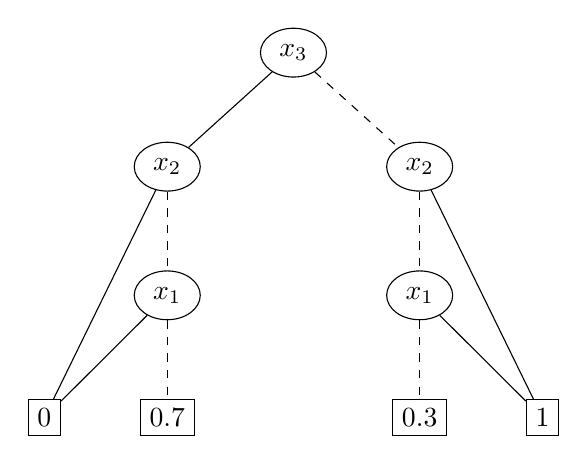
\begin{tikzpicture}
    \node[ellipse,draw] (x3) {$x_3$};
    \node[ellipse,draw,below left = of x3] (x21) {$x_2$};
    \node[ellipse,draw,below right = of x3] (x22) {$x_2$};
    \node[ellipse,draw,below = of x21] (x11) {$x_1$};
    \node[ellipse,draw,below = of x22] (x12) {$x_1$};
    \node[rectangle,draw,below = of x11] (n2) {$0.7$};
    \node[rectangle,draw,left = of n2] (n1) {$0$};
    \node[rectangle,draw,below = of x12] (n3) {$0.3$};
    \node[rectangle,draw,right = of n3] (n4) {$1$};

    \draw (x3) edge (x21);
    \draw (x21) edge (n1);
    \draw (x11) edge (n1);
    \draw[dashed] (x21) edge (x11);
    \draw[dashed] (x11) edge (n2);

    \draw[dashed] (x3) edge (x22);
    \draw[dashed] (x22) edge (x12);
    \draw[dashed] (x12) edge (n3);
    \draw (x22) edge (n4);
    \draw (x12) edge (n4);
  \end{tikzpicture}
\]
Such an ADD for $x_n$ has $2n+3$ nodes and $4n-2$ edges. The same information
can be represented in textual form as
\begin{align*}
  &\texttt{w 3 1 0} \\
  &\texttt{w 3 2 0} \\
  &\texttt{w 3 -1 -2 0.7}
\end{align*}
The encoding weights depend on the probabilities in the CPT as follows. For each
value $x_n$, if $\Pr(X = x_n) = 0$, then $w(x_n) = 0$. Otherwise, let $I_n = \{ 1
\le i \le n - 1 \mid \Pr(X = x_i) \ne 0 \}$. Then
\[
  w \left( x_n \;\middle|\; \bigwedge_{i \in I_n} \neg x_i \right) = \Pr(X =
  x_n) \prod_{i \in I_n} \frac{1}{1 - w \left( x_i \;\middle|\; \bigwedge_{j \in
        I_i} \neg x_j \right)}.
\]
All of these weights/probabilities may have other conditions that come from the
structure of the Bayesian network.

\section{Encoding Bayesian networks}

Let $V$ denote the set of random variables in a Bayesian network. For any random
variable $X \in V$, let $\mathrm{pa}(X)$ denote the set of parents of $X$ and
$\im X$ denote the set of possible values.

\begin{definition}[Indicator variables]
  Let $X \in V$ be a random variable. If $X$ is binary (i.e., $|\im X| = 2$), we
  can arbitrary identify one of the values as $1$ and the other one as $0$ (i.e,
  $\im X \cong \{ 0, 1 \}$). Then $X$ can be represented by a single
  \emph{indicator variable} $\lambda_{X=1}$. If we interpret
  $2^{\{\lambda_{X=1}\}}$ as a Boolean algebra, we can let $\lambda_{X=0} =
  \neg\lambda_{X=1}$ in the algebraic notation, or, equivalently, $\lambda_{X=0}
  = \emptyset \in 2^{\{\lambda_{X=1}\}}$ in the set-theoretic notation. On the
  other hand, if $X$ is not binary, we represent $X$ with $|\im X|$ indicator
  variables, one for each value. We let
  \[
    E(X) = \begin{cases}
      \{ \lambda_{X=1} \} & \text{if } |\im X| = 2 \\
      \{ \lambda_{X=x} \mid x \in \im X \} & \text{otherwise.}
    \end{cases}
  \]
  denote the set of indicator variables for $X$ and
  \[
    E^*(X) = E(X) \cup \bigcup_{Y \in \mathrm{pa}(X)} E(Y).
  \]
  denote the set of indicator variables for $X$ and its parents in the Bayesian
  network. Finally, let
  \[
    U = \bigcup_{X \in V} E(X)
  \]
  denote the set of all indicator variables for all random variables in the
  Bayesian network.
\end{definition}

\begin{definition}[Operations on functions]
  Let $A\colon 2^X \to \mathbb{R}_{\ge 0}$ and $B\colon 2^Y \to \mathbb{R}_{\ge
    0}$ be Boolean functions, $\alpha \in \mathbb{R}_{\ge 0}$, and $x \in X$. We
  define the following operations:
  \begin{description}
  \item[Addition:] $A+B$ is a function $A+B\colon 2^{X \cup Y} \to
    \mathbb{R}_{\ge 0}$ such that
    \[
      (A+B)(\tau) = A(\tau \cap X) + B(\tau \cap Y)
    \]
    for all $\tau \in 2^{X \cup Y}$.
  \item[Inverse:] $\overline{A}$ is a function $\overline{A}\colon 2^X \to
    \mathbb{R}_{\ge 0}$ such that
    \[
      \overline{A}(\tau) = 1 - A(\tau)
    \]
    for all $\tau \in 2^X$.
  \item[Multiplication:] $A \cdot B$ is a function $A \cdot B\colon 2^{X \cup Y}
    \to \mathbb{R}_{\ge 0}$ such that
    \[
      (A \cdot B)(\tau) = A(\tau \cap X) \cdot B(\tau \cap Y)
    \]
    for all $\tau \in 2^{X \cup Y}$.
  \item[Scalar multiplication:] $\alpha A$ is a function $\alpha A\colon 2^X \to
    \mathbb{R}_{\ge 0}$ such that
    \[
      (\alpha A)(\tau) = \alpha \cdot A(\tau)
    \]
    for all $\tau \in 2^X$.
  \item[Projection:] $\exists_xA$ is a function $\exists_xA\colon 2^{X \setminus
      \{ x \}} \to \mathbb{R}_{\ge 0}$ such that
    \[
      (\exists_xA)(\tau) = A(\tau) + A(\tau \cup \{ x \})
    \]
    for all $\tau \in 2^{X \setminus \{x \}}$.
  \end{description}
\end{definition}
Note that both addition and multiplication commute.

\begin{definition}[Special functions]
  \phantom{}
  \begin{itemize}
  \item unit $1\colon 2^\emptyset \to \mathbb{R}_{\ge 0}$, $1(\tau) = 1$.
  \item zero $0\colon 2^\emptyset \to \mathbb{R}_{\ge 0}$, $0(\tau) = 0$.
  \item constant $[a]\colon 2^{\{a\}} \to \mathbb{R}_{\ge 0}$,
    \[
      [a](\tau) =
      \begin{cases}
        1 & \text{if } a \in \tau \\
        0 & \text{if } a \not\in \tau.
      \end{cases}
    \]
  \end{itemize}
\end{definition}

Henceforth, for any function $A\colon 2^X \to \mathbb{R}_{\ge 0}$ and any set
$\tau$, we will write $A(\tau)$ to mean $A(\tau \cap X)$.

\begin{algorithm}
  $\phi \gets 1$\;
  \For{$X \in V$}{
    \textit{let} $\mathrm{pa}(X) = \{ Y_1, \dots, Y_n \}$\;
    $\mathrm{CPT}_X \gets 0$\;
    \eIf{$|\im X| = 2$}{
      \For{$(y_1, \dots, y_n) \in \prod_{i = 1}^n \im Y_i$}{
        $p_1 \gets \Pr(X = 1 \mid Y_1 = y_1, \dots, Y_n = y_n)$\;
        $p_0 \gets \Pr(X \ne 1 \mid Y_1 = y_1, \dots, Y_n = y_n)$\;
        $\mathrm{CPT}_X \gets \mathrm{CPT}_X + p_1[\lambda_{X=1}] \cdot
        \prod_{i=1}^n [\lambda_{Y_i=y_i}] + p_0 \overline{[\lambda_{X=1}]} \cdot
        \prod_{i=1}^n [\lambda_{Y_i=y_i}]$\;
      }
    }{
      \textit{let} $\im X = \{ x_1, \dots, x_m \}$\;
      \For{$x \in \im X$ {\rm \textbf{and}} $(y_1, \dots, y_n) \in \prod_{i =
          1}^n \im Y_i$}{
        $p_x \gets \Pr(X = x \mid Y_1 = y_1, \dots, Y_n = y_n)$\;
        $\mathrm{CPT}_X \gets \mathrm{CPT}_X + p_x[\lambda_{X=x}] \cdot
        \prod_{i=1}^n [\lambda_{Y_i=y_i}] + \overline{[\lambda_{X=1}]} \cdot
        \prod_{i=1}^n [\lambda_{Y_i=y_i}]$\;
      }
      $\mathrm{CPT}_X \gets \mathrm{CPT}_X \cdot \left( \sum_{i=1}^m [\lambda_{X
          = x_i}] \right) \cdot \prod_{i=1}^m \prod_{j=i+1}^m
      (\overline{[\lambda_{X = x_i}]} + \overline{[\lambda_{X = x_j}]})$\;
    }
    $\phi \gets \phi \cdot \mathrm{CPT}_X$\;
  }
  \Return{$\phi$}\;
\end{algorithm}

\begin{lemma} \label{lemma:cpt}
  Let $X \in V$ be a random variable with parents $\mathrm{pa}(X) = \{ Y_1,
  \dots, Y_n \}$. Then $\mathrm{CPT}_X\colon 2^{E^*(X)} \to \mathbb{R}_{\ge 0}$
  is such that for any $x \in \im X$ and $(y_1, \dots, y_n) \in \prod_{i=1}^n
  \im Y_i$,
  \[
    \mathrm{CPT}_X \left( \lambda_{X=x} \land \bigwedge_{i=1}^n
      \lambda_{Y_i=y_i} \right) = \Pr(X = x \mid Y_1 = y_1, \dots, Y_n = y_n).
  \]
\end{lemma}
\begin{proof}
  Let
  \[
    \tau = \lambda_{X=x} \land \bigwedge_{i=1}^n \lambda_{Y_i=y_i}.
  \]
  If $X$ is binary, then $\mathrm{CPT}_X$ is a sum of $2\prod_{i=1}^n |\im Y_i|$
  terms, one for each possible assignment of values to variables $X, Y_1, \dots,
  Y_n$. Exactly one of these terms is nonzero when applied to $\tau$, and it is
  equal to $\Pr(X = x \mid Y_1 = y_1, \dots, Y_n = y_n)$ by definition.

  If $X$ is not binary, then
  \[
    \left( \sum_{i=1}^m [\lambda_{X = x_i}] \right)(\tau) = 1,
  \]
  and
  \[
    \left( \prod_{i=1}^m \prod_{j=i+1}^m (\overline{[\lambda_{X = x_i}]} +
      \overline{[\lambda_{X = x_j}]}) \right)(\tau) = 1,
  \]
  so, by a similar argument as before,
  \[
    \mathrm{CPT}_X(\tau) = \Pr(X = x \mid Y_1 = y_1, \dots, Y_n = y_n).
  \]
\end{proof}

\begin{proposition} \label{lemma:full_distribution}
  $\phi\colon 2^U \to \mathbb{R}_{\ge 0}$ represents the full probability
  distribution of the Bayesian network, i.e., if $V = \{ X_1, \dots, X_n\}$,
  then
  \[
    \phi(\tau) =
    \begin{cases}
      \Pr(X_1 = x_1, \dots, X_n = x_n) & \text{if } \tau = \bigwedge_{i=1}^n
      \lambda_{X_i = x_i} \text{ for some } (x_1, \dots, x_n) \in \prod_{i=1}^n
      \im X_i \\
      0 & \text{otherwise,}
    \end{cases}
  \]
  for all $\tau \in 2^U$.
\end{proposition}
\begin{proof}
  If
  \[
    \tau = \bigwedge_{X \in V} \lambda_{X = v_X}
  \]
  for some $(v_X)_{X \in V} \in \prod_{X \in V} \im X$, then
  \[
    \phi(\tau) = \prod_{X \in V} \Pr \left( X=v_X \;\middle|\; \bigwedge_{Y \in
        \mathrm{pa}(X)} Y=v_Y \right) = \Pr \left( \bigwedge_{X \in V} X=v_X
    \right)
  \]
  by \cref{lemma:cpt} and the definition of a Bayesian network. Otherwise there
  must be some non-binary random variable $X \in V$ such that $|E(X) \cap \tau|
  \ne 1$. If $E(X) \cap \tau = \emptyset$, then
  \[
    \left( \sum_{i=1}^m [\lambda_{X = x_i}] \right)(\tau) = 0,
  \]
  and so $\mathrm{CPT}_X(\tau) = 0$, and $\phi(\tau) = 0$. If $|E(X) \cap
  \tau| > 1$, then we must have two different values $x_1, x_2 \in \im X$ such
  that $\{\lambda_{X=x_1}, \lambda_{X=x_2} \} \subseteq \tau$ which means that
  \[
    (\overline{[\lambda_{X=x_1}]} + \overline{[\lambda_{X=x_2}]})(\tau) = 0,
  \]
  and so, again, $\mathrm{CPT}_X(\tau) = 0$, and $\phi(\tau) = 0$.
\end{proof}

\begin{theorem}
  Let $\phi\colon 2^U \to \mathbb{R}_{\ge 0}$ be a function generated by the
  algorithm. Then
  \[
    (\exists_U(\phi \cdot [\lambda_{X=x}]))(\emptyset) = \Pr(X = x).
  \]
\end{theorem}
\begin{proof}
  Let $V = \{ X, Y_1, \dots, Y_n \}$. Then
  \begin{align*}
    (\exists_U (\phi \cdot [\lambda_{X=x}]))(\emptyset) &= \sum_{\tau \in 2^U} (\phi \cdot [\lambda_{X=x}])(\tau) = \sum_{\lambda_{X=x} \in \tau \in 2^U} \phi(\tau) = \sum_{\lambda_{X=x} \in \tau \in 2^U} \left( \prod_{Y \in V} \mathrm{CPT}_Y \right)(\tau) \\
    &= \sum_{(y_1, \dots, y_n) \in \prod_{i=1}^n \im Y_i} \Pr(X = x, Y_1 = y_1, \dots, Y_n = y_n) = \Pr(X = x)
  \end{align*}
  by the following arguments:
  \begin{itemize}
  \item the proof of Theorem~1 in the ADDMC paper \cite{DBLP:conf/aaai/DudekPV20};
  \item if $\lambda_{X=x} \not\in \tau \in 2^U$, then $(\phi \cdot
    [\lambda_{X=x}])(\tau) = \phi(\tau) \cdot [\lambda_{X=x}](\tau \cap \{
    \lambda_{X=x} \}) = \phi(\tau) \cdot 0 = 0$;
  \item \cref{lemma:full_distribution};
  \item marginalisation of a probability distribution.
  \end{itemize}
\end{proof}

\begin{example}
  \begin{figure}
    \centering
    \begin{subfigure}{0.2\textwidth}
      \centering
      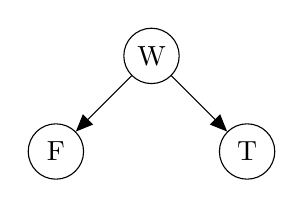
\begin{tikzpicture}
        \node[latent] (W) {W};
        \node[latent, below right=of W] (T) {T};
        \node[latent, below left=of W] (F) {F};
        \edge {W} {F};
        \edge {W} {T};
      \end{tikzpicture}
    \end{subfigure}%
    \begin{subfigure}{0.8\textwidth}
      \centering
      \begin{tabular}[t]{cc}
        \toprule
        $w$ & $\Pr(W = w)$ \\
        \midrule
        1 & 0.5 \\
        0 & 0.5 \\
        \bottomrule
      \end{tabular}
      \begin{tabular}[t]{ccc}
        \toprule
        $w$ & $f$ & $\Pr(F = f \mid W = w)$ \\
        \midrule
        1 & 1 & 0.6 \\
        1 & 0 & 0.4 \\
        0 & 1 & 0.1 \\
        0 & 0 & 0.9 \\
        \bottomrule
      \end{tabular}
      \begin{tabular}[t]{ccc}
        \toprule
        $w$ & $t$ & $\Pr(T = t \mid W = w)$ \\
        \midrule
        1 & $l$ & 0.2 \\
        1 & $m$ & 0.4 \\
        1 & $h$ & 0.4 \\
        0 & $l$ & 0.6 \\
        0 & $m$ & 0.3 \\
        0 & $h$ & 0.1 \\
        \bottomrule
      \end{tabular}
    \end{subfigure}
    \caption{An example Bayesian network with its CPTs}
    \label{fig:example_bn}
  \end{figure}

  The Bayesian network in \cref{fig:example_bn} has
  \begin{align*}
    V &= \{ W, F, T \}, \\
    \mathrm{pa}(W) &= \emptyset, \\
    \mathrm{pa}(F) &= \mathrm{pa}(T) = \{ W \}, \\
    \im W &= \im F = \{ 0, 1 \}, \\
    \im T &= \{ l, m, h \}, \\
    E(W) &= \{ \lambda_{W=1} \}, \\
    E(F) &= \{ \lambda_{F=1} \}, \\
    E(T) &= \{ \lambda_{T=l}, \lambda_{T=m}, \lambda_{T=h} \}, \\
    E^*(W) &= \{ \lambda_{W=1} \}, \\
    E^*(F) &= \{ \lambda_{F=1}, \lambda_{W=1} \}, \\
    E^*(T) &= \{ \lambda_{T=l}, \lambda_{T=m}, \lambda_{T=h}, \lambda_{W=1} \}, \\
    \mathrm{CPT_W} &= 0.5[\lambda_{W=1}]+0.5\overline{[\lambda_{W=1}]} = 0.5 \cdot 1, \\
    \mathrm{CPT_F} &= 0.6[\lambda_{F=1}] \cdot [\lambda_{W=1}] + 0.4[\lambda_{F=0}] \cdot [\lambda_{W=1}] + 0.1[\lambda_{F=1}] \cdot [\lambda_{W=0}] + 0.9[\lambda_{F=0}] \cdot [\lambda_{W=0}] \\
      &= 0.6[\lambda_{F=1}] \cdot [\lambda_{W=1}] + 0.4\overline{[\lambda_{F=1}]} \cdot [\lambda_{W=1}] + 0.1[\lambda_{F=1}] \cdot \overline{[\lambda_{W=1}]} + 0.9\overline{[\lambda_{F=1}]} \cdot \overline{[\lambda_{W=1}]}, \\
    \mathrm{CPT_T} &= ([\lambda_{T=l}] + [\lambda_{T=m}] + [\lambda_{T=h}]) \cdot (\overline{[\lambda_{T=l}]} + \overline{[\lambda_{T=m}]}) \cdot (\overline{[\lambda_{T=l}]} + \overline{[\lambda_{T=h}]}) \cdot (\overline{[\lambda_{T=m}]} + \overline{[\lambda_{T=h}]}) \cdot (\dots),
  \end{align*}
  and can be encoded in a DIMACS-like CNF format as
  \[
    \begin{array}{l r r l l}
      \lambda\sb{T=l} &\lambda\sb{T=m} &\lambda\sb{T=h} & &0 \\
                      &-\lambda\sb{T=l} &-\lambda\sb{T=m} & &0 \\
                      &-\lambda\sb{T=l} &-\lambda\sb{T=h} & &0 \\
                      &-\lambda\sb{T=m} &-\lambda\sb{T=h} & &0 \\
      w &\lambda\sb{W=1} & &0.5 &0.5 \\
      w &\lambda\sb{F=1} &\lambda\sb{W=1} &0.6 &0.4 \\
      w &\lambda\sb{F=1} &-\lambda\sb{W=1} &0.1 &0.9 \\
      w &\lambda\sb{T=l} &\lambda\sb{W=1} &0.2 &1 \\
      w &\lambda\sb{T=m} &\lambda\sb{W=1} &0.4 &1 \\
      w &\lambda\sb{T=h} &\lambda\sb{W=1} &0.4 &1 \\
      w &\lambda\sb{T=l} &\lambda\sb{W=0} &0.6 &1 \\
      w &\lambda\sb{T=m} &\lambda\sb{W=0} &0.3 &1 \\
      w &\lambda\sb{T=h} &\lambda\sb{W=0} &0.1 &1
    \end{array}
  \]
  with each $\lambda$ replaced with a unique positive integer.
\end{example}

\bibliographystyle{plain}
\bibliography{paper}

\end{document}
